\chapter{Instrumentation and experimental setup for SAXS measurements}
\label{chap:experimental_setup}

Since the appearance of third generation facilities, synchrotron radiation sources have become of importance in Small-angle X-ray Scattering experiments due to their high brilliance and collimation, favoring the application of SAXS in a wide variety of scientific fields. The most relevant instrumentation required in a small-angle X-ray scattering experiment are the X-ray source, a sample environment and an area detector which collects the elastic scattered photons. 

The first part of this chapter (section \ref{sec:BESSY}) describes the synchrotron X-ray source, the electron storage ring BESSY II. After this short review on synchrotron radiation, the four-crystal monochromator (FCM) beamline operating in the PTB laboratory at BESSY II is introduced (section \ref{sec:fcm}), where the entirety of the reported results were measured. Following this, the area detector mounted on the HZB-SAXS instrument is reviewed (section \ref{sec:SAXS_experimental}), highlighting the newly developed \emph{in-vacuum} Pilatus X-ray detector and the low uncertainty associated to the sample-detector distance that can be achieved with this setup. Finally, section \ref{sec:sample_environment} presents a detailed insight into the different sample environments needed for the nanoparticles in suspension studied in this work. A brief overview of the data reduction is given in section \ref{sec:data_reduction}, emphasizing the \emph{a posteriori} corrections required by the scattering curve.


\section{Synchrotron radiation at BESSY II}
\label{sec:BESSY}

Synchrotron radiation is the electromagnetic dipole radiation which is emitted by ultra-relativistic charged particles when are accelerated by an external field. The kinetic energy loss of the charged particles (typically electrons) due to the Bremsstrahlung process \citep{blumenthal_bremsstrahlung_1970} is tangentially radiated in form of a light cone with high brilliance and a wide photon energy range. The radiant power of a single relativistic electron in a homogenous magnetic field is expressed by the Larmor formula:

\begin{equation}
        P=\frac{e^2}{6\pi\epsilon_0c}\left( \dot{\beta}^2 + \frac{(\dot{\vec{\beta}} \cdot \vec{\beta})^2}{1-\beta^2} \right) \gamma^4
\end{equation}

where $\vec{\beta}=\frac{\vec{v}}{c}$, the Lorentz factor is $\gamma=\frac{1}{\sqrt{1-\beta^2}}=\frac{E}{m_e c^2}$ and $v$, $m_e$ and $E$ are the velocity, rest mass and energy of the electron respectively.

The total power emitted by an ultra-relativistic electron accelerated radially ($\vec{a} \bot \vec{v}$) is described by:

\begin{equation}
        P_{sync}=\frac{e^2 c}{6\pi\epsilon_0 R^2}\left(\frac{E}{m_e c}\right)^4 \propto E^4 m_e^{-4} R^{-2}
\end{equation}

where $R$ is the radius of the electron trajectory in the circular storage ring and is related to the external magnetic field strength of the bending magnet ($B$) by $R=\frac{E}{ecB}$. The use of light particles (electrons or positrons) in storage rings such as BESSY II is explained by the production of a radiative power $\sim 10^{13}$ times larger than heavier particles like protons.

Synchrotron radiation sources generating X-rays photons have arisen as an important tool in many scientific fields like physical chemistry, life science or physics. The broad spectral range and the high brilliance open new experimental possibilities in materials science as well as in metrology. For instance, the synchrotron radiation can be employed as a primary calibration standard for electromagnetic radiation \citep{thornagel_electron_2001} by means of the Schwinger equation \citep{schwinger_classical_1949} and the determination of the number of electrons per bunch, the electron energy and the magnetic field of the bending magnet.

The two most characteristic features of a synchrotron radiation source are the brilliance and the critical energy or critical wavelength. The brilliance is defined as the number of photons per second, per 100 mA circulating electron current in the storage ring, per electron beam source cross section in mm$^2$, per angular divergence in mrad$^2$, per 0.1 $\% \; \frac{\Delta\lambda}{\lambda}$ \citep{baumgartel_e.-e._1984}, where $\Delta\lambda$ is the bandwidth at a certain wavelength $\lambda$. The critical energy $E_C$ is defined by \citep{schwinger_classical_1949}:

\begin{equation}
        E_C=\frac{3hc}{4\pi R}\left(\frac{E}{m_e c}\right)^3
\end{equation}

The critical energy $E_C$ divides the spectral range into two parts with equal radiated power \citep{baumgartel_e.-e._1984}.

\subsection{The BESSY II Electron Storage Ring}

The facility BESSY II situated in Berlin (Germany) is a synchrotron X-ray and UV light source of third generation. The electrons are accelerated to 1.72 GeV in a booster synchrotron and injected into a storage ring with a 240 m circumference and an electron current of approximately 300 mA \citep{couprie_x_2008}. The following paragraphs describe the creation of X-ray light from the acceleration of the electron beam until the emission of synchrotron radiation on the bending magnets situated along the storage ring \citep{bakker_orbit_1998, bakker_status_1999}.

\begin{figure}%[htbp]
	\centering
		\resizebox{0.4\linewidth}{!}{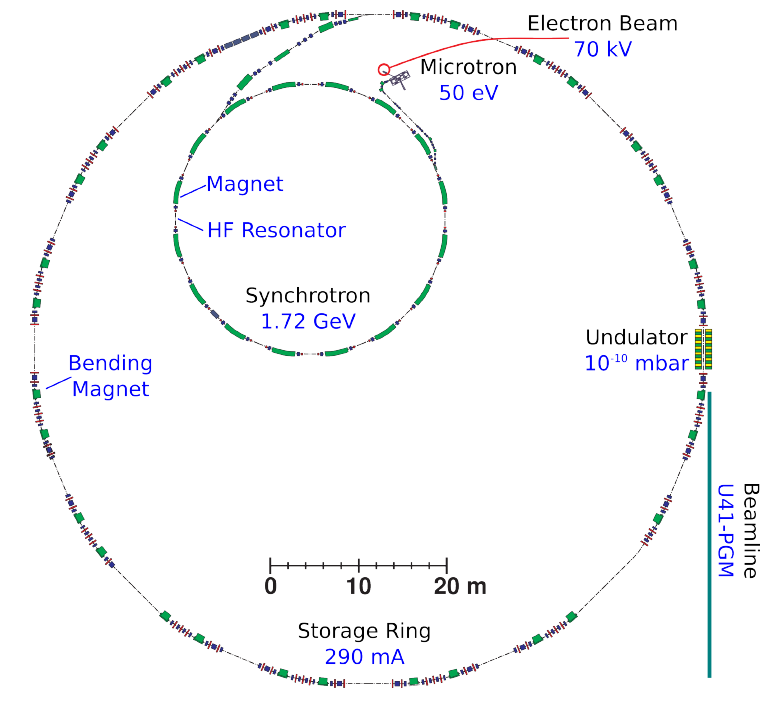
\includegraphics{Figures/BessyScheme.png}}
		\caption{A scheme of BESSY II. From the master thesis.}
		\label{fig:BessyScheme}
\end{figure}


The creation of the free electrons on the electron beam is the first step, as depicted schematically in figure \ref{fig:BessyScheme}. A hot thermionic cathode emits electrons which are accelerated with a high voltage to the anode up to a 70 keV energy and inserted into a linear pre-accelerator, which brings the electron beam to relativistic velocities. The electrons are then transferred into a Scanditronix 50 MeV racetrack microtron (3 GHz) and further accelerated in a 10 Hz booster synchrotron. The acceleration process in the rapid-cycling synchrotron takes about 50 ms and is achieved by the disposition of a set of magnets and 500 MHz rf-cavities coupled with the magnets in linear paths that ramp the electron beam to its final operation energy of 1.72 GeV.

At this point the electrons are injected into the storage ring, where 32 bending magnets with a magnetic field strenght of 1.3 T and a bending radius of 4.2 m \citep{klein_elektronenspeicherringe_2014} are equipped to maintain the circular trajectory of the electron beam at 1.25 MHz revolution frequency. The storage ring has a circumference of 240 meters and the successive injection of electrons from the booster synchrotron leads to currents of approximately 300 mA in the TopUp Mode. The characteristic energy $E_C$ of the bending magnets at BESSY II is 2.5 keV. 

\subsection{Insertion devices}

The synchrotron light sources of third generation such as BESSY II are designed with the goal of optimizing the insertion devices and, therefore, enhance the spectral brightness \citep{ries_nonlinear_2014}. The employment of insertion devices, such as wiggles or undulators, on the straight sections of the storage ring can improve the brilliance or produce light polarizations different from that produced by bending magnets.

Both insertion devices consist on the same principle: a large number ($N\sim100$) of equally spaced alternately polarised dipole magnets stimulate the emission of synchrotron radiation on the experiment direction. By this approach, the photon flux can be increased  in a factor $N$, the number of magnets separated with a spatial field period ($\lambda_0$) in the range of cm. The distinguishable property between wigglers and undulators is their deflection parameter $K$, defined by \citep{baumgartel_e.-e._1984}:

\begin{equation}
        K=\frac{e}{m_e 2\pi c}B_0\lambda_0
\end{equation}

where $B_0$ is the magnetic field amplitude of the dipole magnet. Normally, $K$ can be modified by varying the space between the dipole magnets (\emph{gap}) and, thus, whether the insertion device is  called a wiggler or an undulator depends on its particular configuration. The value of $K$ is rather large in the case of wigglers, emitting radiation in a broad spectral range and increasing the $E_C$ of the storage ring. On the other hand, undulator devices have $K\leq1$, emitting an almost monochromatic and highly intense photon beam.

\section{FCM Beamline}
\label{sec:fcm}

The four-crystal monochromator bending magnet beamline operating in the PTB laboratory at BESSY II \citep{krumrey_design_1998, krumrey_high-accuracy_2001} provides a monochromatic beam in the 1.75-10 keV energy range at a fixed sample position with very high photon flux reproducibility and high energy resolving power. A schematic depiction of the beamline and its components is shown in figure \ref{fig:FCMScheme}.

\begin{figure}%[htbp]
	\centering
		\resizebox{0.8\linewidth}{!}{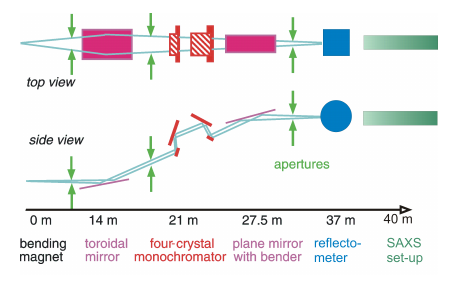
\includegraphics{Figures/FCMScheme.png}}
		\caption{A scheme of the FCM beamline in the PTB laboratory at BESSY II. The distance of each component to the insertion device is shown.}
		\label{fig:FCMScheme}
\end{figure}

At 14 m of the bending magnet, a Pt-coated toroidal mirror is located to focus the beam in the horizontal direction and to collimate it in the vertical direction. The radiation coming from the bending magnet is monochromatised further downstream by a set of 4 single crystals which reflect the light according to the Bragg's law for the (1 1 1) reflexion. As the 4 crystals are mounted on two wheels (one on the rotation center and one parallel aligned), the rotation angle of the wheel ($\Theta$) defines the energy of the outgoing photon beam by $E=\frac{\sqrt{3}h c}{2a\sin{\Theta}}$, where $a$ is the lattice constant of the crystal.

Two types of exchangeable crystal sets, Si ($a=0.543$ nm) and InSb ($a=0.648$ nm), are available to cover the energy range from 1.75 keV to 10 keV. The convolution of the 4 Bragg reflections provides a very high energy resolving power ($E/\Delta E = 10^4 $) through the full energy range. Besides, the geometric disposition of the crystals fixes the position of the outgoing radiation. The monochromator is operated under a $10^{-8}$ mbar vacuum.

The energy range is traced back to the well-known lattice constant of Si. The back-reflection of a silicon crystal at different lattice planes is measured at known energies and the energy is calibrated to the dips positions appearing when the Bragg condition is fulfilled. This approach was employed at the sensitive surface of the X-ray detector introduced in section \ref{sec:pilatus} for an energy range between 4 keV and 10 keV \citep{gollwitzer_diffraction_2014}. To check the accuracy of the energy calibration in a standard measurement, a transmission scan around the K-edge of a copper foil (8980.5 eV) can be measured.

About 10 m before the sample chamber, a bendable plane mirror collimates the beam in the vertical direction and focuses it in the horizontal direction. The mirror is coated with two different materials in separated areas. The Pt-coating is employed to maximize the reflectivity at energies above 4 keV, while the MgF$_2$ supresses the higher orders at energies below 4 keV. The photon flux achieved with the different configurations available at the FCM beamline is shown in figure \ref{fig:FCMBeamlineFlux}, although it can vary depending on the precise disposition of the different apertures along the beam path.

\begin{figure}%[htbp]
	\centering
		% GNUPLOT: LaTeX picture with Postscript
\begingroup
  \makeatletter
  \providecommand\color[2][]{%
    \GenericError{(gnuplot) \space\space\space\@spaces}{%
      Package color not loaded in conjunction with
      terminal option `colourtext'%
    }{See the gnuplot documentation for explanation.%
    }{Either use 'blacktext' in gnuplot or load the package
      color.sty in LaTeX.}%
    \renewcommand\color[2][]{}%
  }%
  \providecommand\includegraphics[2][]{%
    \GenericError{(gnuplot) \space\space\space\@spaces}{%
      Package graphicx or graphics not loaded%
    }{See the gnuplot documentation for explanation.%
    }{The gnuplot epslatex terminal needs graphicx.sty or graphics.sty.}%
    \renewcommand\includegraphics[2][]{}%
  }%
  \providecommand\rotatebox[2]{#2}%
  \@ifundefined{ifGPcolor}{%
    \newif\ifGPcolor
    \GPcolortrue
  }{}%
  \@ifundefined{ifGPblacktext}{%
    \newif\ifGPblacktext
    \GPblacktextfalse
  }{}%
  % define a \g@addto@macro without @ in the name:
  \let\gplgaddtomacro\g@addto@macro
  % define empty templates for all commands taking text:
  \gdef\gplbacktext{}%
  \gdef\gplfronttext{}%
  \makeatother
  \ifGPblacktext
    % no textcolor at all
    \def\colorrgb#1{}%
    \def\colorgray#1{}%
  \else
    % gray or color?
    \ifGPcolor
      \def\colorrgb#1{\color[rgb]{#1}}%
      \def\colorgray#1{\color[gray]{#1}}%
      \expandafter\def\csname LTw\endcsname{\color{white}}%
      \expandafter\def\csname LTb\endcsname{\color{black}}%
      \expandafter\def\csname LTa\endcsname{\color{black}}%
      \expandafter\def\csname LT0\endcsname{\color[rgb]{1,0,0}}%
      \expandafter\def\csname LT1\endcsname{\color[rgb]{0,1,0}}%
      \expandafter\def\csname LT2\endcsname{\color[rgb]{0,0,1}}%
      \expandafter\def\csname LT3\endcsname{\color[rgb]{1,0,1}}%
      \expandafter\def\csname LT4\endcsname{\color[rgb]{0,1,1}}%
      \expandafter\def\csname LT5\endcsname{\color[rgb]{1,1,0}}%
      \expandafter\def\csname LT6\endcsname{\color[rgb]{0,0,0}}%
      \expandafter\def\csname LT7\endcsname{\color[rgb]{1,0.3,0}}%
      \expandafter\def\csname LT8\endcsname{\color[rgb]{0.5,0.5,0.5}}%
    \else
      % gray
      \def\colorrgb#1{\color{black}}%
      \def\colorgray#1{\color[gray]{#1}}%
      \expandafter\def\csname LTw\endcsname{\color{white}}%
      \expandafter\def\csname LTb\endcsname{\color{black}}%
      \expandafter\def\csname LTa\endcsname{\color{black}}%
      \expandafter\def\csname LT0\endcsname{\color{black}}%
      \expandafter\def\csname LT1\endcsname{\color{black}}%
      \expandafter\def\csname LT2\endcsname{\color{black}}%
      \expandafter\def\csname LT3\endcsname{\color{black}}%
      \expandafter\def\csname LT4\endcsname{\color{black}}%
      \expandafter\def\csname LT5\endcsname{\color{black}}%
      \expandafter\def\csname LT6\endcsname{\color{black}}%
      \expandafter\def\csname LT7\endcsname{\color{black}}%
      \expandafter\def\csname LT8\endcsname{\color{black}}%
    \fi
  \fi
  \setlength{\unitlength}{0.0500bp}%
  \begin{picture}(5668.00,4534.00)%
    \gplgaddtomacro\gplbacktext{%
      \csname LTb\endcsname%
      \put(748,704){\makebox(0,0)[r]{\strut{}$10^{10}$}}%
      \csname LTb\endcsname%
      \put(748,3073){\makebox(0,0)[r]{\strut{}$10^{11}$}}%
      \csname LTb\endcsname%
      \put(1039,484){\makebox(0,0){\strut{} 2}}%
      \csname LTb\endcsname%
      \put(1568,484){\makebox(0,0){\strut{} 3}}%
      \csname LTb\endcsname%
      \put(2097,484){\makebox(0,0){\strut{} 4}}%
      \csname LTb\endcsname%
      \put(2626,484){\makebox(0,0){\strut{} 5}}%
      \csname LTb\endcsname%
      \put(3155,484){\makebox(0,0){\strut{} 6}}%
      \csname LTb\endcsname%
      \put(3684,484){\makebox(0,0){\strut{} 7}}%
      \csname LTb\endcsname%
      \put(4213,484){\makebox(0,0){\strut{} 8}}%
      \csname LTb\endcsname%
      \put(4742,484){\makebox(0,0){\strut{} 9}}%
      \csname LTb\endcsname%
      \put(5271,484){\makebox(0,0){\strut{} 10}}%
      \put(176,2486){\rotatebox{-270}{\makebox(0,0){\strut{}Photon flux / s$^{-1}$}}}%
      \put(3075,154){\makebox(0,0){\strut{}Photon Energy / keV}}%
    }%
    \gplgaddtomacro\gplfronttext{%
      \csname LTb\endcsname%
      \put(4284,4096){\makebox(0,0)[r]{\strut{}InSb(111) / MgF$_2$}}%
      \csname LTb\endcsname%
      \put(4284,3876){\makebox(0,0)[r]{\strut{}Si(111) / Pt}}%
      \csname LTb\endcsname%
      \put(4284,3656){\makebox(0,0)[r]{\strut{}Si(111) / MgF$_2$}}%
    }%
    \gplbacktext
    \put(0,0){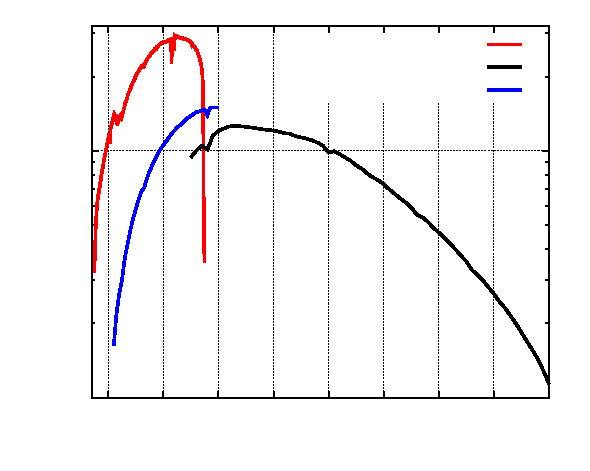
\includegraphics{FCMBeamlineFlux}}%
    \gplfronttext
  \end{picture}%
\endgroup

		\caption{Photon flux of the FCM beamline using different crystals (InSb(111) and Si(111)) and mirror coatings (MgF$_2$ and Pt) at standard operation (300 mA).}
		\label{fig:FCMBeamlineFlux}
\end{figure}

The first slit behind the bending magnet is used to limit the acceptance angle of the radiation into the monochromator. Two moveable slits more are employed downstream to block the parasitic scattering. The 8 $\mu$m thick silicon photodiode can be used for energies above 3 keV. A germanium 520 $\mu$m circular pinhole (Scatex, Incoatec, Geesthacht, Germany) situated before the sample chamber shapes the photon beam into a circular spot on the sample and strongly reduces the parasitic radiation. A flux monitor diode is equipped behind these components and can measure continuously the incoming photon flux.

\subsection{UHV X-ray Reflectometer}

The sample chamber is situated 37 m away from the insertion device, right behind the flux monitor diode. The UHV X-ray Reflectometer disposes of a large volume (60 cm diameter and 70 cm length) which is fully evacuated to reach pressures of approximately $10^{-7}$ mbar. High vacuum is needed to perform experiments at the low energies accessible at the FCM beamline, as the attenuation length of air at energies below 2 keV is less than 1 cm. A smaller lock chamber connected to the sample chamber by a small flange is used to exchange samples without breaking the vacuum of the larger UHV X-ray reflectometer.

The motors of the sample holder can be moved linearly along 3 axes perpendicular to the incoming beam and with very high precision and reproducibility. The broad range of the $x$-motor (160 mm) permits the measurement of different sample capillaries (ca. 20) at once without ventilating the chamber for exchanging the sample.

The large volume of the reflectometer provides enough space to allocate other components close to the sample holder. For example, about 10 cm before the sample position, a 1 mm circular guard pinhole (Incoatec, Geesthacht, Germany) is equipped to remove the parasitic scattering resulting from the collimating system. Behind the sample, the transmitted radiation is measured with a (10 x 10) mm$^2$ silicon photodiode. The thick Can500C diode (Canberra, Meriden, USA) is capable of measuring through the entire beamline energy range, from 1.75 keV to 10 keV, and is calibrated against a cryogenic electric substitution radiometer with a relative uncertainty of \( 1\,\% \) \cite{krumrey_high-accuracy_2001}.

\section{SAXS Setup}
\label{sec:SAXS_experimental}

The intensity scattered by the sample is recorded at a certain distance behind the sample (sample-detector distance) with an area X-ray detector mounted on the HZB SAXS instrument and connected to the sample chamber. Typically, long sample-detector distances are required to access the small angles employed in SAXS experiments.

\subsection{X-ray area detector}
\label{sec:pilatus}

The scattered X-ray photons are collected by a large-area hybrid pixel detector. The Pilatus 1M (Dectris Ltd, Baden, Switzerland) has a sensitive surface of (179 x 169) mm$^2$ and consists of a silicon pixel matrix with a pixel size of $d = (172.1 \pm 0.2)$ $\mu$m which operates in single-photon counting mode, providing very low darkcount rates and signal-to-noise ratios and a high dynamic range. For instance, the detector quantum efficiency is about 97 $\%$ at 8 keV using the ultra-high gain mode and almost 86 $\%$ at 4 keV \citep{wernecke_characterization_2014}.

Besides, the Pilatus 1M detector was modified to operate under vacuum to cover the full energetic range available at the beamline, down to 1.75 keV. The windowless detector is directly connected to the sample chamber with an evacuated bellow and cooled down at 5-10$^{\circ}$C. The narrow point-spread function of the detector and the available low energies increase the momentum transfer resolution and the accessible $q$-range.

A moveable beamstop mounted at thin wires is installed just in front of the detector to block the intense transmitted photon beam, avoiding saturation effects in the central pixels. The beamstop is constructed within a funnel-like cavity ($\oslash$ 5 mm) to reduce geometrically the reflections on the beamstop surface, which are damped by the cavity. A silicon photodiode with a sensitive area of (2.5 x 2.5) mm$^2$ (S10356-01, Hamamatsu, Shizuoka, Japan) covers the beamstop to monitor the sample transmission during the experiment, revealing the possible radiation damage of the sample.

\subsection{HZB SAXS instrument and WAXS configuration}

The in-vacuum Pilatus 1M detector is mounted on the SAXS instrument of the Helmholtz-Zentrum Berlin (HZB), which is connected via a $\oslash$100 mm flange to the UHV X-ray Reflectometer. The HZB-SAXS apparatus is equipped with a large below system and a motorized stage that can vary the sample-detector distance continuously between 2.3 m and 4.6 m in vacuum (about $10^{-4}$ mbar) with an uncertainty of 20 $\mu$m. 

Complementary to the HZB-SAXS instrument, the sample-detector distance can be reduced down to about 760 mm by attaching the X-ray detector directly to the sample chamber, increasing the scattering angles to around $8^{\circ}$. This short-distance setup, or Wide-angle X-ray Scattering (WAXS) configuration, is used for the study of nanoparticles with diameters below 10 nm, whose characteristic features appear beyond 1 nm$^{-1}$. The accessible $q$-range of this setup is summarized in table \ref{tab:qrange} for the high-energy case, which provides the highest $q$-value available. Similarly, the table shows the limit $q$-values achieved with the HZB-SAXS apparatus at low-energy.

\begin{table}[]
\centering
\caption{Accessible $q$-range for the different experimental setups at the low and high energy limits.}
\label{tab:qrange}
\begin{tabular}{|l|c|c|}
\hline
              & \textbf{SAXS} & \textbf{WAXS} \\ \hline
Distance (mm) & 4540          & 760           \\ \hline
Energy (eV)   & 4000          & 10000         \\ \hline
$q_{min}$ (nm$^{-1}$)   & \textbf{0.015}         & 0.2          \\ \hline
$q_{max}$ (nm$^{-1}$)   & 0.56             & \textbf{7}             \\ \hline
\end{tabular}
\end{table}

\subsubsection{Calibration of the sample-detector distance}

In small-angle scattering experiments, it is crucial to know precisely the distance between the irradiated sample and the detector, in order to calibrate the momentum transfer $q$. Typically, a calibration standard material with a well-known crystal lattice parameter is employed, which produces well-defined diffraction rings in the low-angle region. A material extensively used is dry rat-tail tendon collagen, with a $d$-spacing of 650 \AA \citep{amenitsch_performance_1997}, corresponding to $q=0.097$ nm$^{-1}$. The degradation of this material upon prolonged radiation suggested the use of harder calibrants such as silver behenate (CH$_3$(CH$_2$)$_{20}$COO$\cdot$Ag) \citep{huang_x-ray_1993}.

AgBehe has a very narrow diffraction ring at $q=1.0763$ nm$^{-1}$, arising from a long-period spacing ($d_{001]}$) value of 58.36 \AA \citep{blanton_jcpdsinternational_1995}, although this value depends slightly on the synthesis. A deviation of 0.5 $\%$ in the diffraction peak position could be observed for different sample preparations. In order to increase the accuracy of the calibration, the sample-detector distance was determined by the detection of the scattering pattern of AgBehe at different positions of the HZB SAXS instrument, measured with the built-in 3 m long Heidenhain optical encoder. By triangulating the radius of the diffraction ring to the source point, as depicted in figure \ref{fig:DistanceCalibrationSAXS}, the sample-detector distance is obtained in a traceable way.

\begin{figure}
	\centering
	        \subfloat[Distance Calibration]{\resizebox{0.5\linewidth}{!}{% GNUPLOT: LaTeX picture with Postscript
\begingroup
  \makeatletter
  \providecommand\color[2][]{%
    \GenericError{(gnuplot) \space\space\space\@spaces}{%
      Package color not loaded in conjunction with
      terminal option `colourtext'%
    }{See the gnuplot documentation for explanation.%
    }{Either use 'blacktext' in gnuplot or load the package
      color.sty in LaTeX.}%
    \renewcommand\color[2][]{}%
  }%
  \providecommand\includegraphics[2][]{%
    \GenericError{(gnuplot) \space\space\space\@spaces}{%
      Package graphicx or graphics not loaded%
    }{See the gnuplot documentation for explanation.%
    }{The gnuplot epslatex terminal needs graphicx.sty or graphics.sty.}%
    \renewcommand\includegraphics[2][]{}%
  }%
  \providecommand\rotatebox[2]{#2}%
  \@ifundefined{ifGPcolor}{%
    \newif\ifGPcolor
    \GPcolortrue
  }{}%
  \@ifundefined{ifGPblacktext}{%
    \newif\ifGPblacktext
    \GPblacktextfalse
  }{}%
  % define a \g@addto@macro without @ in the name:
  \let\gplgaddtomacro\g@addto@macro
  % define empty templates for all commands taking text:
  \gdef\gplbacktext{}%
  \gdef\gplfronttext{}%
  \makeatother
  \ifGPblacktext
    % no textcolor at all
    \def\colorrgb#1{}%
    \def\colorgray#1{}%
  \else
    % gray or color?
    \ifGPcolor
      \def\colorrgb#1{\color[rgb]{#1}}%
      \def\colorgray#1{\color[gray]{#1}}%
      \expandafter\def\csname LTw\endcsname{\color{white}}%
      \expandafter\def\csname LTb\endcsname{\color{black}}%
      \expandafter\def\csname LTa\endcsname{\color{black}}%
      \expandafter\def\csname LT0\endcsname{\color[rgb]{1,0,0}}%
      \expandafter\def\csname LT1\endcsname{\color[rgb]{0,1,0}}%
      \expandafter\def\csname LT2\endcsname{\color[rgb]{0,0,1}}%
      \expandafter\def\csname LT3\endcsname{\color[rgb]{1,0,1}}%
      \expandafter\def\csname LT4\endcsname{\color[rgb]{0,1,1}}%
      \expandafter\def\csname LT5\endcsname{\color[rgb]{1,1,0}}%
      \expandafter\def\csname LT6\endcsname{\color[rgb]{0,0,0}}%
      \expandafter\def\csname LT7\endcsname{\color[rgb]{1,0.3,0}}%
      \expandafter\def\csname LT8\endcsname{\color[rgb]{0.5,0.5,0.5}}%
    \else
      % gray
      \def\colorrgb#1{\color{black}}%
      \def\colorgray#1{\color[gray]{#1}}%
      \expandafter\def\csname LTw\endcsname{\color{white}}%
      \expandafter\def\csname LTb\endcsname{\color{black}}%
      \expandafter\def\csname LTa\endcsname{\color{black}}%
      \expandafter\def\csname LT0\endcsname{\color{black}}%
      \expandafter\def\csname LT1\endcsname{\color{black}}%
      \expandafter\def\csname LT2\endcsname{\color{black}}%
      \expandafter\def\csname LT3\endcsname{\color{black}}%
      \expandafter\def\csname LT4\endcsname{\color{black}}%
      \expandafter\def\csname LT5\endcsname{\color{black}}%
      \expandafter\def\csname LT6\endcsname{\color{black}}%
      \expandafter\def\csname LT7\endcsname{\color{black}}%
      \expandafter\def\csname LT8\endcsname{\color{black}}%
    \fi
  \fi
    \setlength{\unitlength}{0.0500bp}%
    \ifx\gptboxheight\undefined%
      \newlength{\gptboxheight}%
      \newlength{\gptboxwidth}%
      \newsavebox{\gptboxtext}%
    \fi%
    \setlength{\fboxrule}{0.5pt}%
    \setlength{\fboxsep}{1pt}%
\begin{picture}(5668.00,4534.00)%
    \gplgaddtomacro\gplbacktext{%
      \csname LTb\endcsname%
      \put(264,2622){\makebox(0,0)[r]{\strut{}$300$}}%
      \csname LTb\endcsname%
      \put(264,3067){\makebox(0,0)[r]{\strut{}$400$}}%
      \csname LTb\endcsname%
      \put(264,3511){\makebox(0,0)[r]{\strut{}$500$}}%
      \csname LTb\endcsname%
      \put(264,3955){\makebox(0,0)[r]{\strut{}$600$}}%
      \csname LTb\endcsname%
      \put(264,4399){\makebox(0,0)[r]{\strut{}$700$}}%
      \csname LTb\endcsname%
      \put(618,2047){\makebox(0,0){\strut{}}}%
      \csname LTb\endcsname%
      \put(1726,2047){\makebox(0,0){\strut{}}}%
      \csname LTb\endcsname%
      \put(2834,2047){\makebox(0,0){\strut{}}}%
      \csname LTb\endcsname%
      \put(3941,2047){\makebox(0,0){\strut{}}}%
      \csname LTb\endcsname%
      \put(5049,2047){\makebox(0,0){\strut{}}}%
    }%
    \gplgaddtomacro\gplfronttext{%
      \csname LTb\endcsname%
      \put(-242,3509){\rotatebox{-270}{\makebox(0,0){\strut{}Radius size / pixel}}}%
      \csname LTb\endcsname%
      \put(1314,4234){\makebox(0,0)[r]{\strut{}AgBehe}}%
      \csname LTb\endcsname%
      \put(1314,3904){\makebox(0,0)[r]{\strut{}SBA}}%
    }%
    \gplgaddtomacro\gplbacktext{%
      \csname LTb\endcsname%
      \put(264,721){\makebox(0,0)[r]{\strut{}$-3$}}%
      \csname LTb\endcsname%
      \put(264,1036){\makebox(0,0)[r]{\strut{}$-2$}}%
      \csname LTb\endcsname%
      \put(264,1352){\makebox(0,0)[r]{\strut{}$-1$}}%
      \csname LTb\endcsname%
      \put(264,1667){\makebox(0,0)[r]{\strut{}$0$}}%
      \csname LTb\endcsname%
      \put(264,1983){\makebox(0,0)[r]{\strut{}$1$}}%
      \csname LTb\endcsname%
      \put(618,343){\makebox(0,0){\strut{}2500}}%
      \csname LTb\endcsname%
      \put(1726,343){\makebox(0,0){\strut{}3000}}%
      \csname LTb\endcsname%
      \put(2834,343){\makebox(0,0){\strut{}3500}}%
      \csname LTb\endcsname%
      \put(3941,343){\makebox(0,0){\strut{}4000}}%
      \csname LTb\endcsname%
      \put(5049,343){\makebox(0,0){\strut{}4500}}%
    }%
    \gplgaddtomacro\gplfronttext{%
      \csname LTb\endcsname%
      \put(-209,1305){\rotatebox{-270}{\makebox(0,0){\strut{}Residuals / pixel}}}%
      \put(2833,46){\makebox(0,0){\strut{}Measured distance / mm}}%
    }%
    \gplbacktext
    \put(0,0){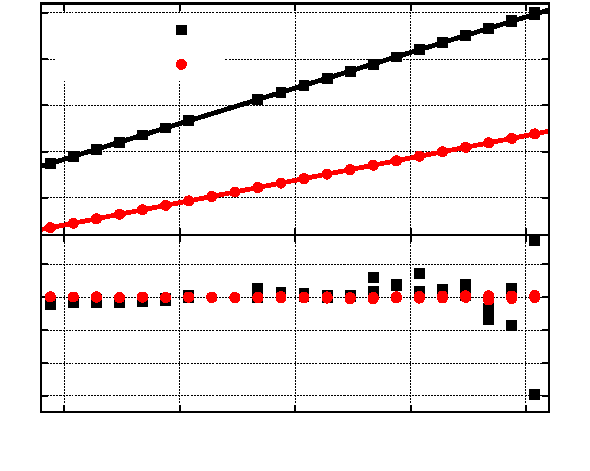
\includegraphics{DistanceCalibrationSAXS}}%
    \gplfronttext
  \end{picture}%
\endgroup
}\label{fig:DistanceCalibrationSAXS}}
		\subfloat[AgBehe at large distance]{\resizebox{0.35\linewidth}{!}{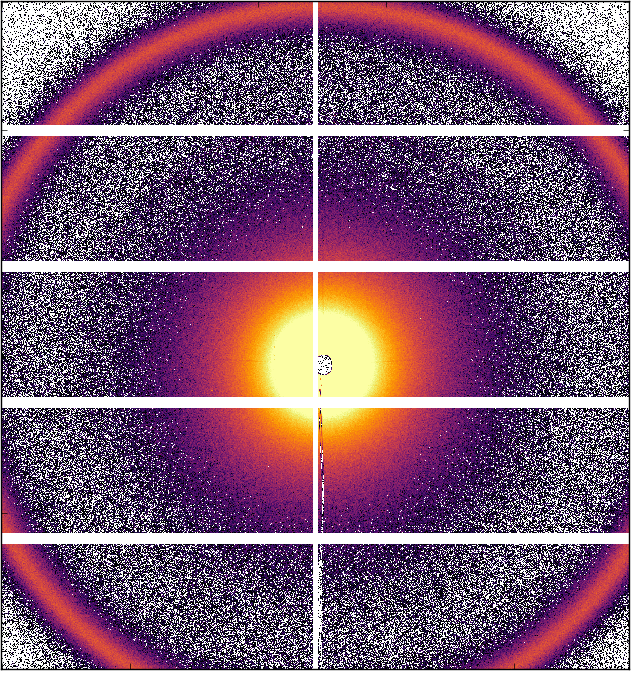
\includegraphics{Figures/AgBeheSAXSLongDistance_edit.png}}\label{fig:AgBeheSAXSLongDistance}}
		\caption{Sample-to-detector distance calibration: a) Radius of the diffraction ring of AgBehe and SBA-15 as a function of the sample-detector distance. A linear function is fitted to obtain the source point distance. The residuals of the fitting are shown in the bottom plot. b) Scattering pattern of AgBehe measured at a distance of 3638.2 mm. The diffraction rings exceeds the detector area. \textcolor{red}{file "messung kmc daten 2015 1Q pilatus 201501 0394.tif"}}
\end{figure}

By measuring the AgBehe pattern along a distance range of 2200 mm with 100 mm steps at 8000 eV, the relative uncertainty associated to the linear fitting is 0.03 $\%$, corresponding to 1.5 mm. As observed in the residuals of the fitting in figure \ref{fig:DistanceCalibrationSAXS}, the deviation increases for long distances, due to the relatively small $d$-spacing of AgBehe, disabling the use of distances larger than $\sim 3600$ mm. In figure \ref{fig:AgBeheSAXSLongDistance}, it is visible how the diffraction ring surpasses the surface of the detector at a distance of 3638.2 mm and, thus, diminishes the accuracy of the peak determination.

By using a material with lower $q$-value, such as the templated mesoporous silica SBA-15 \citep{zhao_triblock_1998} ($q=0.681$ nm$^{-1}$), this limitation can be mitigated as shown in figure \ref{fig:DistanceCalibrationSAXS}, where the residuals of SBA are minimal for the entire distance range. By using SBA and increasing the accessible distance range, the relative uncertainty of the fit decreases in a factor 5, reaching an uncertainty of 0.004 $\%$ (0.2 mm) when measuring with 50 mm steps. This improvement is also related with the narrower diffraction peak of SBA-15 (FWHM/$q=2.6\%$) in comparison to AgBehe ($5.5\%$).

Although the fit uncertainty is smaller in the SBA case, the position and shape of diffraction peak depend strongly on the sample preparation (e.g. template pore size). For the same polymer template, the $q$-value of the ring can vary until 1 $\%$ for different thermal treatments and radiation damage effects are visible for short calcination times. On the other side, prolonged beam exposure of AgBehe can damage the sample as well and create small silver nanoparticles, which increase the scattering background \cite{liu_thermal_2006}. The choice of the calibration standard depends strictly on the needs of the experiment. Besides, the largest contributions to the sample-detector distance uncertainty come from the thickness of the sample (ca. 0.5 mm) and from the difference between the calibration with AgBehe and SBA-15 (also 0.5 mm). Normally the uncertainty associated with the distance calibration is $10^{-4}$, similar to the energy resolving power described in section \ref{sec:fcm}.

\section{Sample environment}
\label{sec:sample_environment}

The sample consists normally of a few microliters of nanoparticles in solution which are measured in a vacuum-proof container positioned inside the reflectometer. The sample environment must fulfill some requirements:

\begin{itemize}
        \item The container's material should minimize the innecessary absorption of the X-ray photon flux by the sample environment.
        \item The container volume should be small enough to enable the measurement of valuable, limited samples.
        \item The optimal sample thickness for a transmission diffraction experiment is the inverse of its attenuation coefficient $\mu(E)$, which reduces the incoming intensity to $\sim37\%$. For example, the optimal thickness of water at 8000 eV is around 1 mm.
\end{itemize}

Typically, the samples are introduced in thin glass capillaries which maintain the temperature and pressure of the sample close to the ambient conditions. However, there are different sample environments which can be used depending on the requirements of the experiment. In this work, only nanoparticles suspended in aqueous media have been employed, allowing the use of a similar attenuation coefficient for almost all experiments.

\subsection{Round capillaries}

For single-contrast SAXS measurements, borosilicate glass 3.3 round capillaries of 100 mm length were used. They were purchased at WJM Glass (Berlin, Germany) and had a nominal inner diameter of 1 mm and a wall thickness of 10 $\mu$m. The sample is filled into the capillary with a long syringe (Sterican$\textregistered$21 x 4 3/4" , Braun, Melsungen, Germany), avoiding the contact of the needle with the capillary walls. The top end of the capillary is closed by welding.

The very narrow glass walls (with a density of about 2.23 g cm$^{-3}$) absorb only 14 $\%$ of the incoming flux at 8000 eV and produce very low incoherent scattering background. Therefore, these capillaries are suitable for standard SAXS measurements. Unfortunately, the capillaries sample thickness shows a significant deviation along the vertical axis and are inappropriate for measurements at different capillary heights, as needed for the continuous contrast variation technique.

\subsection{Rectangular capillaries}

The capillaries used for the contrast variation experiments are vacuum-proof borosilicate glass capillaries from Hilgenberg (Malsfeld, Germany) with a nominal rectangular cross section of (4.2 $\pm$ 0.2) x (1.25 $\pm$ 0.05) mm$^2$ , a length of (80 $\pm$ 0.5) mm and a wall thickness of ca. 120 $\mu$m. The thicker glass walls reduce the transmitted intensity about $80\%$ at 8000 eV, but in contrast both the glass and sample thicknesses are very homogenous for the entire capillary.

\begin{figure}%[htbp]
	\centering
		\subfloat[Glass thickness]{\resizebox{0.44\linewidth}{!}{% GNUPLOT: LaTeX picture with Postscript
\begingroup
  \makeatletter
  \providecommand\color[2][]{%
    \GenericError{(gnuplot) \space\space\space\@spaces}{%
      Package color not loaded in conjunction with
      terminal option `colourtext'%
    }{See the gnuplot documentation for explanation.%
    }{Either use 'blacktext' in gnuplot or load the package
      color.sty in LaTeX.}%
    \renewcommand\color[2][]{}%
  }%
  \providecommand\includegraphics[2][]{%
    \GenericError{(gnuplot) \space\space\space\@spaces}{%
      Package graphicx or graphics not loaded%
    }{See the gnuplot documentation for explanation.%
    }{The gnuplot epslatex terminal needs graphicx.sty or graphics.sty.}%
    \renewcommand\includegraphics[2][]{}%
  }%
  \providecommand\rotatebox[2]{#2}%
  \@ifundefined{ifGPcolor}{%
    \newif\ifGPcolor
    \GPcolortrue
  }{}%
  \@ifundefined{ifGPblacktext}{%
    \newif\ifGPblacktext
    \GPblacktextfalse
  }{}%
  % define a \g@addto@macro without @ in the name:
  \let\gplgaddtomacro\g@addto@macro
  % define empty templates for all commands taking text:
  \gdef\gplbacktext{}%
  \gdef\gplfronttext{}%
  \makeatother
  \ifGPblacktext
    % no textcolor at all
    \def\colorrgb#1{}%
    \def\colorgray#1{}%
  \else
    % gray or color?
    \ifGPcolor
      \def\colorrgb#1{\color[rgb]{#1}}%
      \def\colorgray#1{\color[gray]{#1}}%
      \expandafter\def\csname LTw\endcsname{\color{white}}%
      \expandafter\def\csname LTb\endcsname{\color{black}}%
      \expandafter\def\csname LTa\endcsname{\color{black}}%
      \expandafter\def\csname LT0\endcsname{\color[rgb]{1,0,0}}%
      \expandafter\def\csname LT1\endcsname{\color[rgb]{0,1,0}}%
      \expandafter\def\csname LT2\endcsname{\color[rgb]{0,0,1}}%
      \expandafter\def\csname LT3\endcsname{\color[rgb]{1,0,1}}%
      \expandafter\def\csname LT4\endcsname{\color[rgb]{0,1,1}}%
      \expandafter\def\csname LT5\endcsname{\color[rgb]{1,1,0}}%
      \expandafter\def\csname LT6\endcsname{\color[rgb]{0,0,0}}%
      \expandafter\def\csname LT7\endcsname{\color[rgb]{1,0.3,0}}%
      \expandafter\def\csname LT8\endcsname{\color[rgb]{0.5,0.5,0.5}}%
    \else
      % gray
      \def\colorrgb#1{\color{black}}%
      \def\colorgray#1{\color[gray]{#1}}%
      \expandafter\def\csname LTw\endcsname{\color{white}}%
      \expandafter\def\csname LTb\endcsname{\color{black}}%
      \expandafter\def\csname LTa\endcsname{\color{black}}%
      \expandafter\def\csname LT0\endcsname{\color{black}}%
      \expandafter\def\csname LT1\endcsname{\color{black}}%
      \expandafter\def\csname LT2\endcsname{\color{black}}%
      \expandafter\def\csname LT3\endcsname{\color{black}}%
      \expandafter\def\csname LT4\endcsname{\color{black}}%
      \expandafter\def\csname LT5\endcsname{\color{black}}%
      \expandafter\def\csname LT6\endcsname{\color{black}}%
      \expandafter\def\csname LT7\endcsname{\color{black}}%
      \expandafter\def\csname LT8\endcsname{\color{black}}%
    \fi
  \fi
  \setlength{\unitlength}{0.0500bp}%
  \begin{picture}(5668.00,4534.00)%
    \gplgaddtomacro\gplbacktext{%
    }%
    \gplgaddtomacro\gplfronttext{%
      \csname LTb\endcsname%
      \put(1241,736){\makebox(0,0){\strut{}-2}}%
      \put(1625,736){\makebox(0,0){\strut{}-1.5}}%
      \put(2009,736){\makebox(0,0){\strut{}-1}}%
      \put(2393,736){\makebox(0,0){\strut{}-0.5}}%
      \put(2777,736){\makebox(0,0){\strut{} 0}}%
      \put(3160,736){\makebox(0,0){\strut{} 0.5}}%
      \put(3544,736){\makebox(0,0){\strut{} 1}}%
      \put(3928,736){\makebox(0,0){\strut{} 1.5}}%
      \put(4312,736){\makebox(0,0){\strut{} 2}}%
      \put(4696,736){\makebox(0,0){\strut{} 2.5}}%
      \put(2834,406){\makebox(0,0){\strut{}Horizontal Position / mm}}%
      \put(801,1022){\makebox(0,0)[r]{\strut{} 5}}%
      \put(801,1304){\makebox(0,0)[r]{\strut{} 5.5}}%
      \put(801,1587){\makebox(0,0)[r]{\strut{} 6}}%
      \put(801,1869){\makebox(0,0)[r]{\strut{} 6.5}}%
      \put(801,2152){\makebox(0,0)[r]{\strut{} 7}}%
      \put(801,2433){\makebox(0,0)[r]{\strut{} 7.5}}%
      \put(801,2715){\makebox(0,0)[r]{\strut{} 8}}%
      \put(801,2998){\makebox(0,0)[r]{\strut{} 8.5}}%
      \put(801,3280){\makebox(0,0)[r]{\strut{} 9}}%
      \put(801,3563){\makebox(0,0)[r]{\strut{} 9.5}}%
      \put(207,2377){\rotatebox{-270}{\makebox(0,0){\strut{}Vertical Position / mm}}}%
      \put(5107,1022){\makebox(0,0)[l]{\strut{}-2}}%
      \put(5107,1473){\makebox(0,0)[l]{\strut{}-1.5}}%
      \put(5107,1925){\makebox(0,0)[l]{\strut{}-1}}%
      \put(5107,2377){\makebox(0,0)[l]{\strut{}-0.5}}%
      \put(5107,2828){\makebox(0,0)[l]{\strut{} 0}}%
      \put(5107,3280){\makebox(0,0)[l]{\strut{} 0.5}}%
      \put(5107,3732){\makebox(0,0)[l]{\strut{} 1}}%
      \put(5701,2377){\rotatebox{270}{\makebox(0,0){\strut{}Deviation /$\%$}}}%
    }%
    \gplbacktext
    \put(0,0){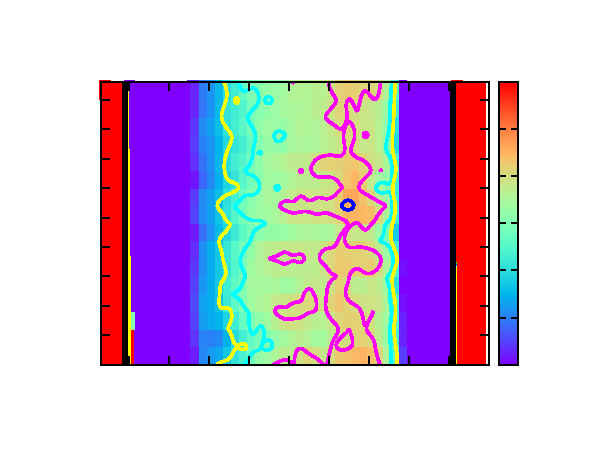
\includegraphics{HilgenbergHomogeneity}}%
    \gplfronttext
  \end{picture}%
\endgroup
}\label{fig:HilgenbergHomogeneity}}
		\subfloat[Sample thickness]{\resizebox{0.44\linewidth}{!}{% GNUPLOT: LaTeX picture with Postscript
\begingroup
  \makeatletter
  \providecommand\color[2][]{%
    \GenericError{(gnuplot) \space\space\space\@spaces}{%
      Package color not loaded in conjunction with
      terminal option `colourtext'%
    }{See the gnuplot documentation for explanation.%
    }{Either use 'blacktext' in gnuplot or load the package
      color.sty in LaTeX.}%
    \renewcommand\color[2][]{}%
  }%
  \providecommand\includegraphics[2][]{%
    \GenericError{(gnuplot) \space\space\space\@spaces}{%
      Package graphicx or graphics not loaded%
    }{See the gnuplot documentation for explanation.%
    }{The gnuplot epslatex terminal needs graphicx.sty or graphics.sty.}%
    \renewcommand\includegraphics[2][]{}%
  }%
  \providecommand\rotatebox[2]{#2}%
  \@ifundefined{ifGPcolor}{%
    \newif\ifGPcolor
    \GPcolortrue
  }{}%
  \@ifundefined{ifGPblacktext}{%
    \newif\ifGPblacktext
    \GPblacktextfalse
  }{}%
  % define a \g@addto@macro without @ in the name:
  \let\gplgaddtomacro\g@addto@macro
  % define empty templates for all commands taking text:
  \gdef\gplbacktext{}%
  \gdef\gplfronttext{}%
  \makeatother
  \ifGPblacktext
    % no textcolor at all
    \def\colorrgb#1{}%
    \def\colorgray#1{}%
  \else
    % gray or color?
    \ifGPcolor
      \def\colorrgb#1{\color[rgb]{#1}}%
      \def\colorgray#1{\color[gray]{#1}}%
      \expandafter\def\csname LTw\endcsname{\color{white}}%
      \expandafter\def\csname LTb\endcsname{\color{black}}%
      \expandafter\def\csname LTa\endcsname{\color{black}}%
      \expandafter\def\csname LT0\endcsname{\color[rgb]{1,0,0}}%
      \expandafter\def\csname LT1\endcsname{\color[rgb]{0,1,0}}%
      \expandafter\def\csname LT2\endcsname{\color[rgb]{0,0,1}}%
      \expandafter\def\csname LT3\endcsname{\color[rgb]{1,0,1}}%
      \expandafter\def\csname LT4\endcsname{\color[rgb]{0,1,1}}%
      \expandafter\def\csname LT5\endcsname{\color[rgb]{1,1,0}}%
      \expandafter\def\csname LT6\endcsname{\color[rgb]{0,0,0}}%
      \expandafter\def\csname LT7\endcsname{\color[rgb]{1,0.3,0}}%
      \expandafter\def\csname LT8\endcsname{\color[rgb]{0.5,0.5,0.5}}%
    \else
      % gray
      \def\colorrgb#1{\color{black}}%
      \def\colorgray#1{\color[gray]{#1}}%
      \expandafter\def\csname LTw\endcsname{\color{white}}%
      \expandafter\def\csname LTb\endcsname{\color{black}}%
      \expandafter\def\csname LTa\endcsname{\color{black}}%
      \expandafter\def\csname LT0\endcsname{\color{black}}%
      \expandafter\def\csname LT1\endcsname{\color{black}}%
      \expandafter\def\csname LT2\endcsname{\color{black}}%
      \expandafter\def\csname LT3\endcsname{\color{black}}%
      \expandafter\def\csname LT4\endcsname{\color{black}}%
      \expandafter\def\csname LT5\endcsname{\color{black}}%
      \expandafter\def\csname LT6\endcsname{\color{black}}%
      \expandafter\def\csname LT7\endcsname{\color{black}}%
      \expandafter\def\csname LT8\endcsname{\color{black}}%
    \fi
  \fi
  \setlength{\unitlength}{0.0500bp}%
  \begin{picture}(5668.00,4534.00)%
    \gplgaddtomacro\gplbacktext{%
    }%
    \gplgaddtomacro\gplfronttext{%
      \csname LTb\endcsname%
      \put(1241,736){\makebox(0,0){\strut{}-2}}%
      \put(2009,736){\makebox(0,0){\strut{}-1}}%
      \put(2777,736){\makebox(0,0){\strut{} 0}}%
      \put(3544,736){\makebox(0,0){\strut{} 1}}%
      \put(4312,736){\makebox(0,0){\strut{} 2}}%
      \put(2834,406){\makebox(0,0){\strut{}Horizontal Position / mm}}%
      \put(801,1323){\makebox(0,0)[r]{\strut{}-4}}%
      \put(801,1926){\makebox(0,0)[r]{\strut{}-2}}%
      \put(801,2527){\makebox(0,0)[r]{\strut{} 0}}%
      \put(801,3130){\makebox(0,0)[r]{\strut{} 2}}%
      \put(801,3732){\makebox(0,0)[r]{\strut{} 4}}%
      \put(471,2377){\rotatebox{-270}{\makebox(0,0){\strut{}Vertical Position / mm}}}%
      \put(5107,1473){\makebox(0,0)[l]{\strut{} 0.99}}%
      \put(5107,2377){\makebox(0,0)[l]{\strut{} 1}}%
      \put(5107,3280){\makebox(0,0)[l]{\strut{} 1.01}}%
      \put(5833,2377){\rotatebox{270}{\makebox(0,0){\strut{}Sample Thickness / mm}}}%
    }%
    \gplbacktext
    \put(0,0){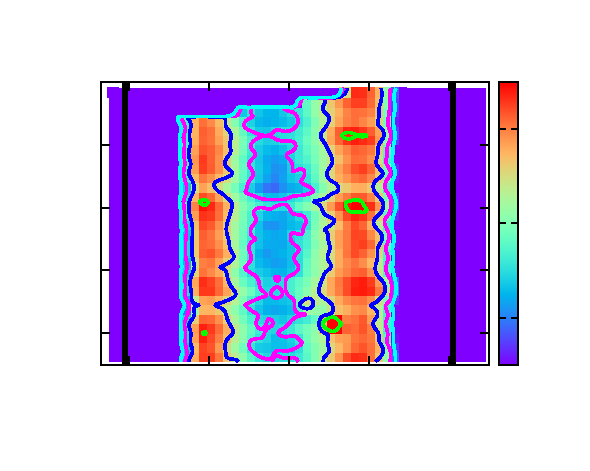
\includegraphics{WaterHomogeneity}}%
    \gplfronttext
  \end{picture}%
\endgroup
}\label{fig:WaterHomogeneity}}
		\caption{Homogeneity of the rectangular capillaries: a) Deviation of the empty capillary tranmission, i.e. glass wall thickness, b) Sample thickness calculated from the water transmission of a filled capillary. }
\end{figure}

The transmission of an empty capillary is mapped in figure \ref{fig:HilgenbergHomogeneity}, where it can be observed that the deviation of the glass wall thickness is less than 2 $\%$ for an horizontal range of 2.5 mm (of a total width of 4.2 mm). This range is at least 5 times larger than the typical beam diameter, avoiding the convolution of different thicknesses in the measurement. Similarly, figure \ref{fig:WaterHomogeneity} depicts the sample thickness in the capillary, calculated from a capillary filled with water using the Beer-Lambert law, the glass transmission and the mass attenuation coefficient of water at 8000 eV, 10.37 cm$^{2}$ g$^{-1}$ \citep{hubbell_tables_1996}. The thickness of the sample introduced in the capillary is homogenous within 2 $\%$ for a width range of ca. 2.5 mm. 

\begin{figure}%[htbp]
	\centering
		% GNUPLOT: LaTeX picture with Postscript
\begingroup
  \makeatletter
  \providecommand\color[2][]{%
    \GenericError{(gnuplot) \space\space\space\@spaces}{%
      Package color not loaded in conjunction with
      terminal option `colourtext'%
    }{See the gnuplot documentation for explanation.%
    }{Either use 'blacktext' in gnuplot or load the package
      color.sty in LaTeX.}%
    \renewcommand\color[2][]{}%
  }%
  \providecommand\includegraphics[2][]{%
    \GenericError{(gnuplot) \space\space\space\@spaces}{%
      Package graphicx or graphics not loaded%
    }{See the gnuplot documentation for explanation.%
    }{The gnuplot epslatex terminal needs graphicx.sty or graphics.sty.}%
    \renewcommand\includegraphics[2][]{}%
  }%
  \providecommand\rotatebox[2]{#2}%
  \@ifundefined{ifGPcolor}{%
    \newif\ifGPcolor
    \GPcolortrue
  }{}%
  \@ifundefined{ifGPblacktext}{%
    \newif\ifGPblacktext
    \GPblacktextfalse
  }{}%
  % define a \g@addto@macro without @ in the name:
  \let\gplgaddtomacro\g@addto@macro
  % define empty templates for all commands taking text:
  \gdef\gplbacktext{}%
  \gdef\gplfronttext{}%
  \makeatother
  \ifGPblacktext
    % no textcolor at all
    \def\colorrgb#1{}%
    \def\colorgray#1{}%
  \else
    % gray or color?
    \ifGPcolor
      \def\colorrgb#1{\color[rgb]{#1}}%
      \def\colorgray#1{\color[gray]{#1}}%
      \expandafter\def\csname LTw\endcsname{\color{white}}%
      \expandafter\def\csname LTb\endcsname{\color{black}}%
      \expandafter\def\csname LTa\endcsname{\color{black}}%
      \expandafter\def\csname LT0\endcsname{\color[rgb]{1,0,0}}%
      \expandafter\def\csname LT1\endcsname{\color[rgb]{0,1,0}}%
      \expandafter\def\csname LT2\endcsname{\color[rgb]{0,0,1}}%
      \expandafter\def\csname LT3\endcsname{\color[rgb]{1,0,1}}%
      \expandafter\def\csname LT4\endcsname{\color[rgb]{0,1,1}}%
      \expandafter\def\csname LT5\endcsname{\color[rgb]{1,1,0}}%
      \expandafter\def\csname LT6\endcsname{\color[rgb]{0,0,0}}%
      \expandafter\def\csname LT7\endcsname{\color[rgb]{1,0.3,0}}%
      \expandafter\def\csname LT8\endcsname{\color[rgb]{0.5,0.5,0.5}}%
    \else
      % gray
      \def\colorrgb#1{\color{black}}%
      \def\colorgray#1{\color[gray]{#1}}%
      \expandafter\def\csname LTw\endcsname{\color{white}}%
      \expandafter\def\csname LTb\endcsname{\color{black}}%
      \expandafter\def\csname LTa\endcsname{\color{black}}%
      \expandafter\def\csname LT0\endcsname{\color{black}}%
      \expandafter\def\csname LT1\endcsname{\color{black}}%
      \expandafter\def\csname LT2\endcsname{\color{black}}%
      \expandafter\def\csname LT3\endcsname{\color{black}}%
      \expandafter\def\csname LT4\endcsname{\color{black}}%
      \expandafter\def\csname LT5\endcsname{\color{black}}%
      \expandafter\def\csname LT6\endcsname{\color{black}}%
      \expandafter\def\csname LT7\endcsname{\color{black}}%
      \expandafter\def\csname LT8\endcsname{\color{black}}%
    \fi
  \fi
  \setlength{\unitlength}{0.0500bp}%
  \begin{picture}(5668.00,4534.00)%
    \gplgaddtomacro\gplbacktext{%
      \csname LTb\endcsname%
      \put(858,921){\makebox(0,0)[r]{\strut{} 0.07}}%
      \put(858,1964){\makebox(0,0)[r]{\strut{} 0.1}}%
      \put(858,3149){\makebox(0,0)[r]{\strut{} 0.15}}%
      \put(858,3990){\makebox(0,0)[r]{\strut{} 0.2}}%
      \put(1275,484){\makebox(0,0){\strut{}-4}}%
      \put(1846,484){\makebox(0,0){\strut{}-2}}%
      \put(2417,484){\makebox(0,0){\strut{} 0}}%
      \put(2988,484){\makebox(0,0){\strut{} 2}}%
      \put(3559,484){\makebox(0,0){\strut{} 4}}%
      \put(4129,484){\makebox(0,0){\strut{} 6}}%
      \put(4700,484){\makebox(0,0){\strut{} 8}}%
      \put(5271,484){\makebox(0,0){\strut{} 10}}%
      \put(220,2486){\rotatebox{-270}{\makebox(0,0){\strut{}Transmission}}}%
      \put(3130,154){\makebox(0,0){\strut{}Vertical position / mm}}%
    }%
    \gplgaddtomacro\gplfronttext{%
      \csname LTb\endcsname%
      \put(2475,3730){\makebox(0,0)[r]{\strut{}Transmission}}%
      \csname LTb\endcsname%
      \put(2475,3510){\makebox(0,0)[r]{\strut{}Glass only}}%
      \csname LTb\endcsname%
      \put(2475,3290){\makebox(0,0)[r]{\strut{}H$_2$O}}%
    }%
    \gplbacktext
    \put(0,0){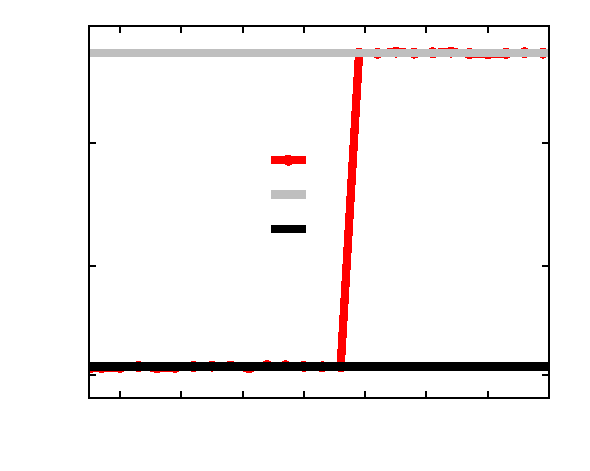
\includegraphics{GaldenCalibration}}%
    \gplfronttext
  \end{picture}%
\endgroup

		\caption{X-ray transmission of a rectangular capillary half-filled with water along the main vertical axis situated at $x=-0.15$ mm.}
		\label{fig:GaldenCalibration}
\end{figure}

From these figures, it is clear that the homogeneity of the sample environment is even better along the main vertical axis of the capillary. Figure \ref{fig:GaldenCalibration} shows the measured X-ray transmission of a half-filled capillary along its vertical axis (at the horizontal position -0.15 mm). For example, the glass transmission within a 6 mm vertical range is $20.1\%$, with an associated relative uncertainty of $\delta_r T =0.6 \; \%$. By calculating $\delta_r d = \frac{\delta_r T}{log(T)}$ where $T$ is the glass transmission, the relative uncertainty of the glass thickness is $\delta_r d = 0.4 \; \%$. Analogously, the uncertainty of the water transmission is 0.9 $\%$ and the sample thicknes has an uncertainty of 0.9 $\%$ along the vertical axis.

These rectangular capillaries are a very suitable sample environment for measurements which require a high homogeneity along the vertical axis of the capillary. The thickness of the wall varies only 0.4 $\%$ and the sample thickness less than 0.9 $\%$, although the thick glass walls reduce considerably the transmitted intensity and produce larger background scattering than the round capillaries.

\subsection{Cell for low-energies}

Samples with larger structures require the measurement of scattering curves at lower $q$-values. To extend the measurable $q$-range, one possibility is to reduce the photon beam energy, though this involves reducing the sample thickness, due to the short penetration length of X-rays at low energies. Therefore, a custom-made sample holder is used utilizing silicon-nitride windows (NX7150E, Norcada Inc., Edmonton, Canada). The 500 nm thickness windows produce very low scattering and have a negligable absorbance ($<5\;\%$) for energies above 4000 eV.

A polymeric 100 $\mu$m ring cut with a microtome is used as spacer between the 2 windows, in order to achieve the desired 120 $\mu$m sample thickness which optimizes the intensity attenuation at 4000 eV. The acces to smaller $q$-values using this cell is shown in \cite{varga_towards_2014}, where a value of $q=0.015$ nm$^{-1}$ is achieved.

\begin{figure}%[htbp]
	\centering
		\resizebox{0.7\linewidth}{!}{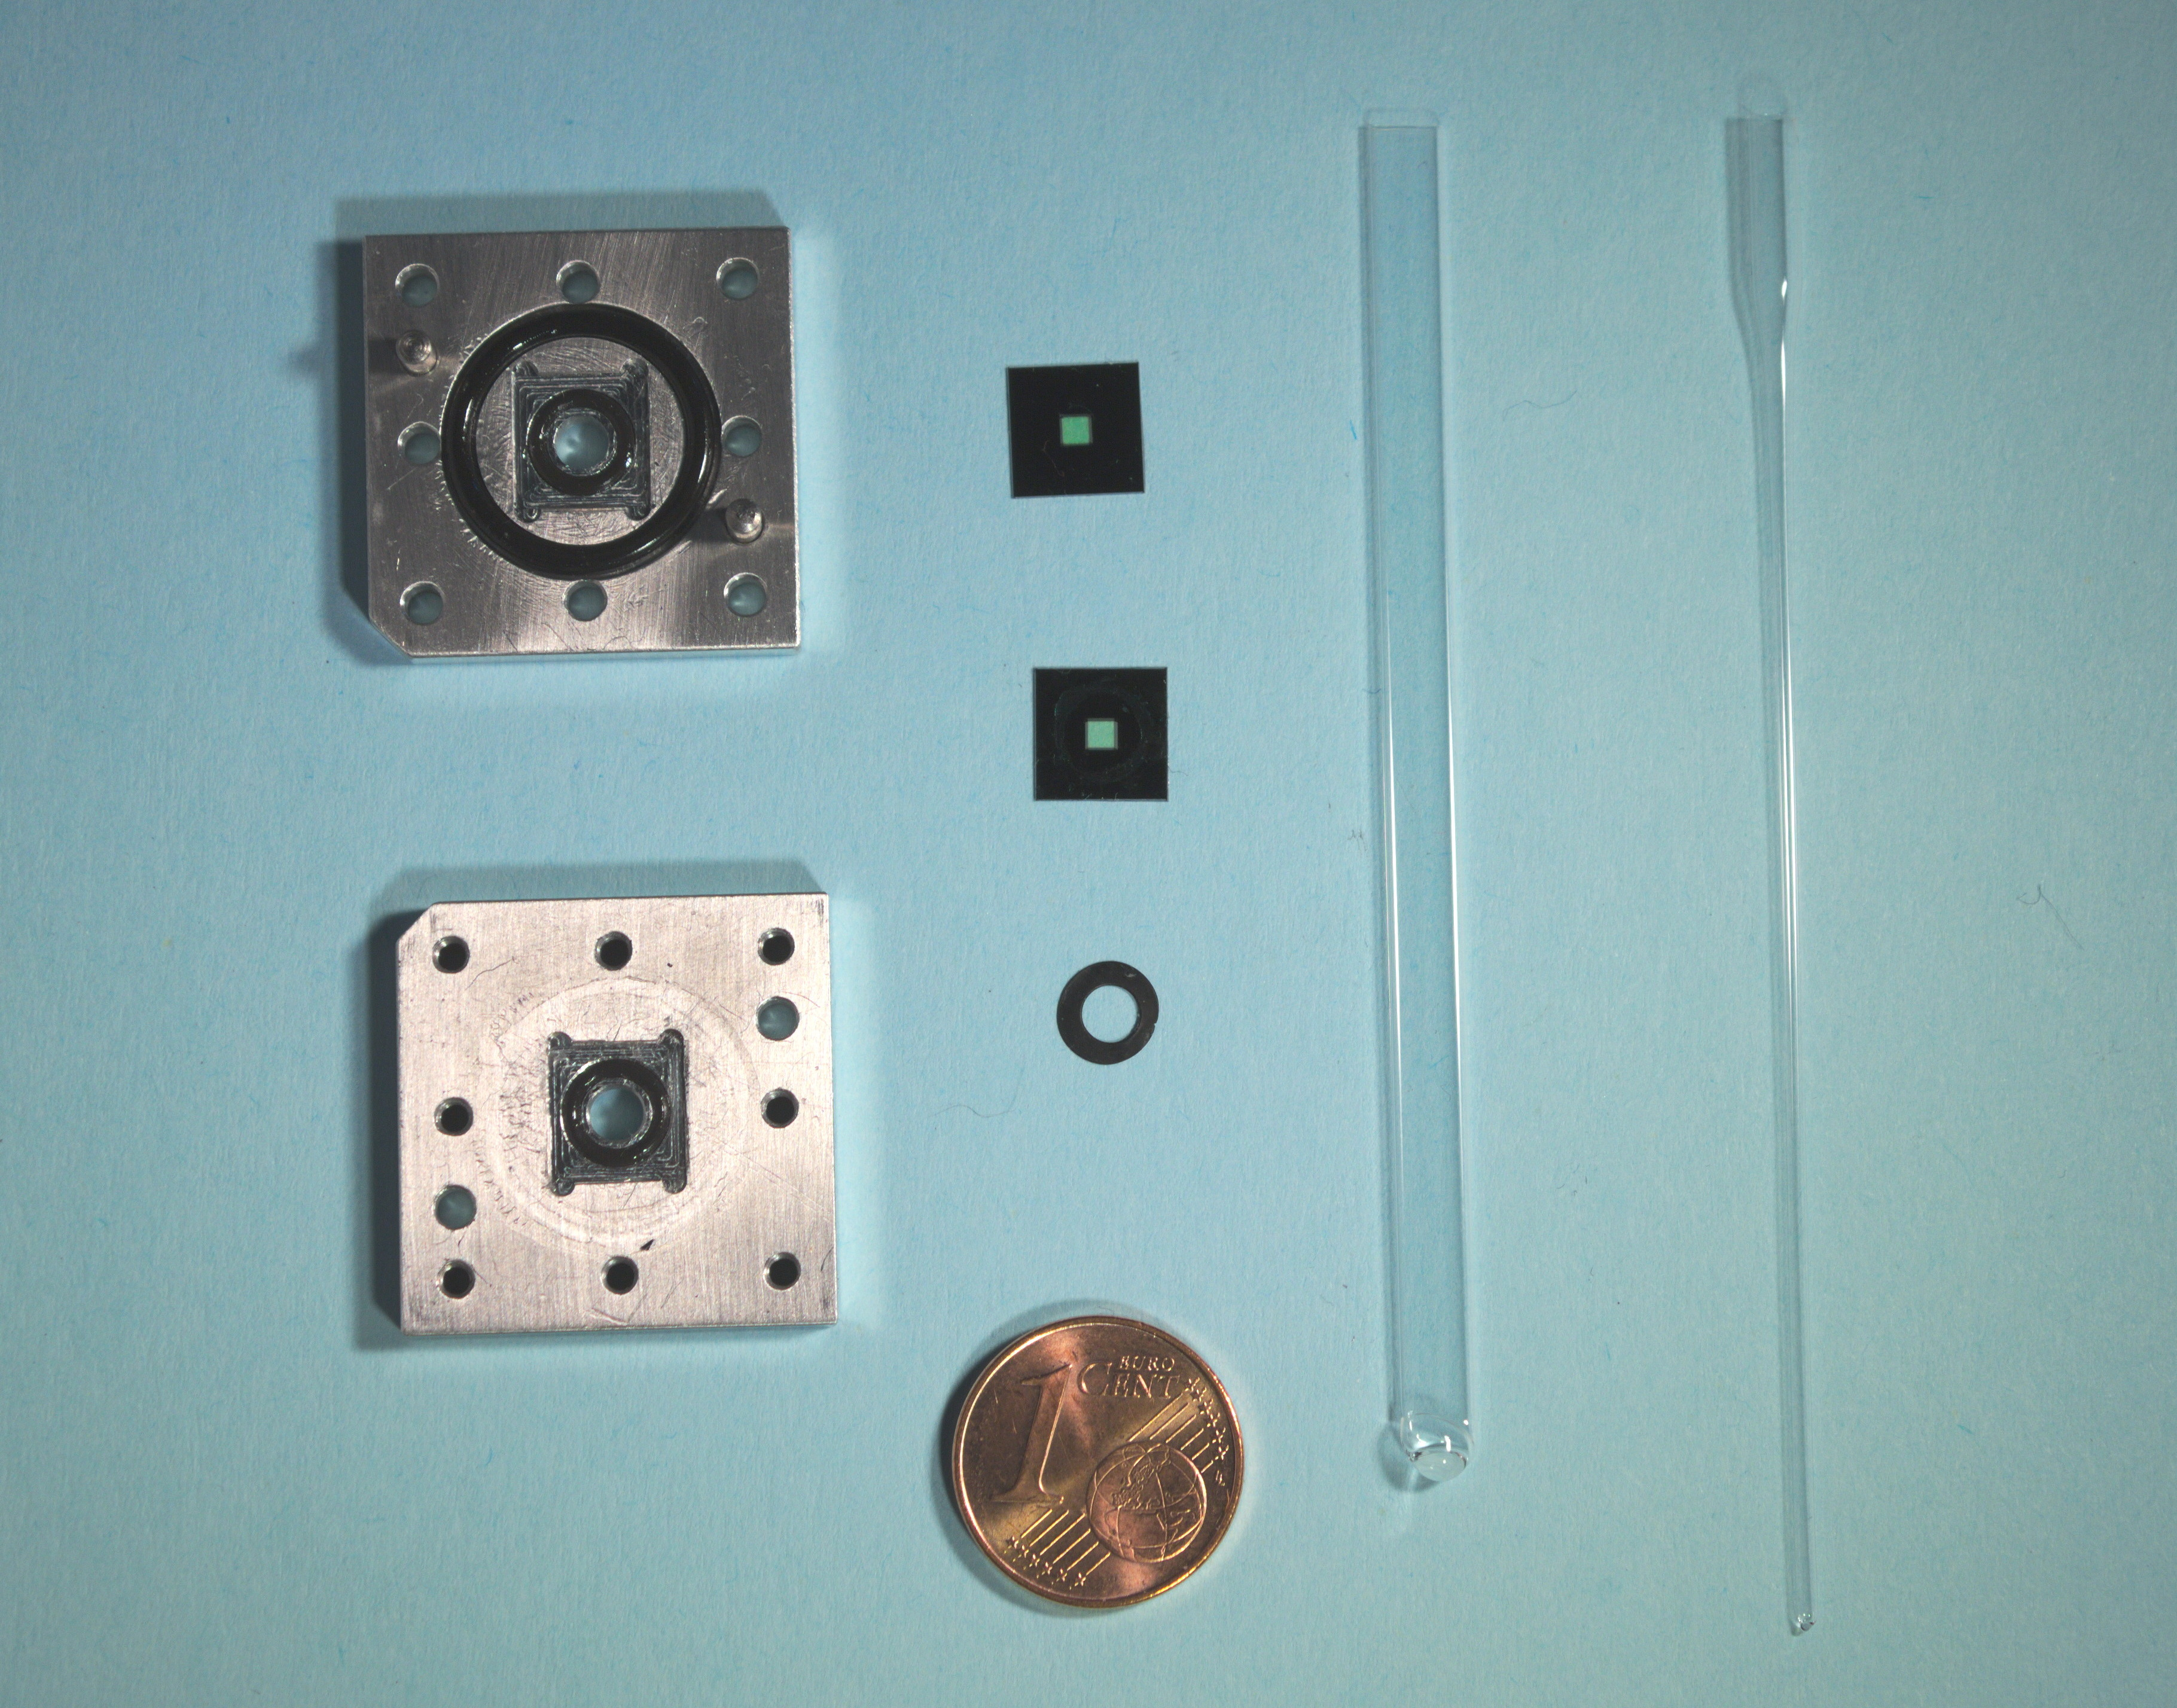
\includegraphics{Figures/SampleEnvironment.jpg}}
		\caption{Different sample environments: On the left side, the disassembled low-energy cell with the two silicon-nitride windows, the polymeric ring spacer and the two parts of the metallic holder. On the right side, the round and rectangular capillaries.}
		\label{fig:SampleEnvironment}
\end{figure}

\section{Data reduction: The scattering curve}
\label{sec:data_reduction}

For isotropically scattering samples e.g. nanoparticles in suspension, the scattering patterns collected in the area detector consist of concentric rings whose center is the transmitted beam. The dimensionality of the data can be reduced by performing a radial integration of the measured pattern, converting the 2D images into 1D scattering curves. This reduction step is based on the $q$-binning: the grouping of pixels with similar scattering angle $q$ irrespective of their azimuthal angle on the detector \citep{pauw_everything_2013}. By averaging the scattered intensity of the pixels within the same $q$-bin ($I(q)$), the uncertainty of the data decreases in the scattering curve. The size of the bins depends on the requirements of the data evaluation while the bins are typically spaced uniformly, although logarithmic distributions are also extensively used. The difference in solid angle for each pixel due to the spherical projection of the scattering on a flat detector is also considered in this step.

The uncertainty associated to the intensity $I(q)$ is calculated as the standard deviation between each pixel intensity in the $q$-bin, which gives a better estimate than the uncertainty associated to the photon-counting Poisson statistics \citep{pauw_everything_2013}. The pixels discarded (or \emph{masked out}) for the weighted average of the $n$th $q$-bin ($q_n$) are those whose intensity is not comprised within the range 

\begin{equation}
\left[ \frac{\left|I_{med}\left( q_{n-1}\right)-I_{med}\left( q_{n}\right)\right|}{2} - 3 \sigma , \frac{\left|I_{med}\left( q_{n+1}\right)-I_{med}\left( q_{n}\right)\right|}{2} + 3 \sigma \right], 
\end{equation}

where $I_{med}\left( q_{n}\right)$ is the median intensity of the pixels prior to this \emph{masking procedure} and $\sigma$ is the standard deviation. With a confidence level of 99.7 $\%$, the pixels excluded of the reduction process are those pixels whose intensity lies clearly out of the radial average, such as \emph{hot pixels}, anisotropic scattering from the glass capillary or undesired reflexes without radial simmetry.

The position of the center of the scattering pattern is of vital importance for the radial integration step. A standard calibrant with very narrow diffraction rings such as AgBehe can be used to locate the center with high precision. Nevertheless, the masking process previously described can be used as well to determine the center position by minimizing the number of masked pixels and the standard deviation uncertainty of the $q$-bins. The accuracy of the center determination is sub-pixel using both approaches, but the masking procedure does not require of a calibration standard material.

The scattering curve obtained by radial integration still requires of some data correction. For instance, $I_{meas}(q)$ (photon counts) must be normalized to the exposure time $\Delta t$, the solid angle $\Delta \Omega$, the measured transmittance of the sample $T$ and the incident photon flux $\Phi_0$, measured by the flux monitor described in section \ref{sec:fcm}. In order to present the scattering cross section per volume $\frac{d\sigma}{d\Omega}/V$ in absolute units (cm$^{-1}$), the measured intensity must be normalized to the sample thickness $t$ and the quantum efficiencies of the X-ray detector and the silicon diodes $\eta_{QE}$: 

\begin{equation}
\frac{\frac{d\sigma}{d\Omega}}{V} \left(q\right)=\frac{I_{meas}\left(q\right)}{\Phi_0 \cdot T \cdot \Delta\Omega \cdot \Delta t \cdot \eta_{QE} \cdot t}
\end{equation}

By using the monitor diode on the beamstop as described in section \ref{sec:pilatus}, $T$ and $\Phi_0$ can be measured simultaneously during the experiment, without the necessity of the flux monitor diode.

Alternatively a standard material like lupolen \cite{kratky_absolute_1966,shaffer_calibration_1974} or glassy carbon \cite{perret_glassy_1972} can be employed to scale the measured scattering intensity to the known values of these materials.

The normalized scattering curve requires of an accurate background correction. The scattering of the pure suspending medium and the sample environment can affect the evaluation of the data, specially for low-scatterers, and, therefore, the normalized scattering background must be subtracted to obtain a usable scattering curve.
